\section{Analisi sintattica: linguaggi liberi}
I linguaggi liberi da contesto (detti anche context-free languages, o CFL) sono una classe di linguaggi formali che possono essere descritti da una grammatica libera da contesto. \red{Questi linguaggi sono più complessi dei linguaggi regolari}, ma non sono generali quanto i linguaggi Turing-completi

\[
        \text{Linguaggi Regolari} \subseteq \text{Linguaggi Liberi}
\]

Questo perché \red{le grammatiche libere da contesto più generali di quelle regolari}:
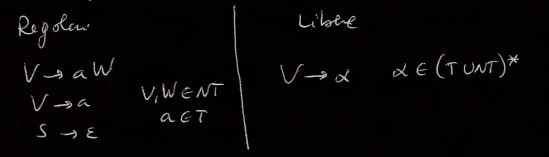
\includegraphics[width=10cm]{gram_libere_regolari.png}

i linguaggi liberi da contesto necessitano, per essere riconosciuti, dei cosiddetti \red{automi a pila} (utilizzano una memoria a "pila" per memorizzare informazioni) al posto dei normali NFA - DFA. Questi PDS si dividono in:
\begin{itemize}
    \item PDA non deterministici sono più potenti e possono riconoscere linguaggi liberi da contesto
    \item PDA deterministici sono meno potenti ma utili per costruire compilatori
\end{itemize}  
\subsection{Analisi sintattica}

\textbf{l'analisi sintattica} è una fase chiave nella compilazione e nell'interpretazione del codice sorgente. Qui viene \red{descritto come un analizzatore sintattico} (\textbf{parser}) \red{processi una lista di token, generata in precedenza dall'analisi lessicale, per produrre un} \textbf{albero di derivazione}

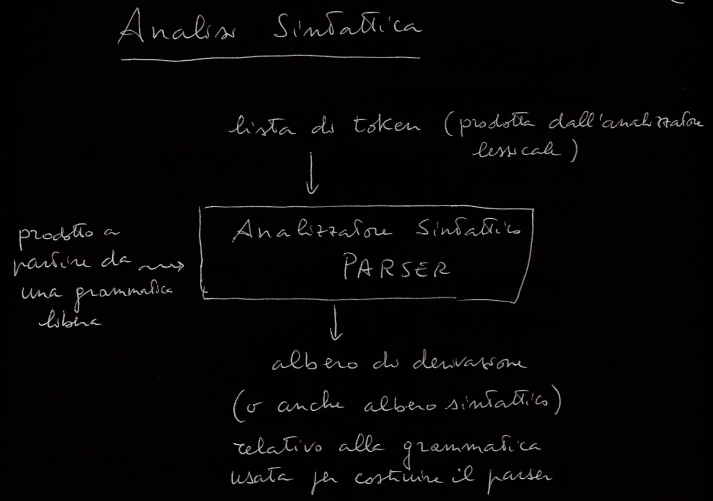
\includegraphics[width=10cm]{analizzatore_sintattico.png}

\subsection{PDA - i riconoscitori dei linguaggi liberi}

Per i linguaggi liberi serve una memoria che ricorda certi input precedenti

\esempio{
    \[
        L=\{ww^r|w\in \{a,b\}^*\}       
    \]
    Dove $L$ è libero perché $L=L(G)$ con $G[S\to \epsilon | aSa|bSb]$ libera. Si ha che:
    \[
        L = L=\{\epsilon, aa, bb, aaaa, abba, baab, bbbb, \dots\}    
    \]
}

Qui infatti l'automa deve ricordarsi della prima metà dell'input per restituire la seconda metà dell'output, ecco che ci verranno in aiuto i \textbf{PDA}
\section{Automi a pila}
\subsection{automi a pila non deterministici}
\definizione{
    un automa a pila non deterministico (PDA) è una 7-upla $(\Sigma, Q, \Gamma, \delta, q_0, \bot, F)$ dove:
    \begin{itemize}
        \item $\Sigma$ è un alfabeto finito 
        \item $Q$ è un insieme finito di stati
        \item $\Gamma$ è un insieme finito di simboli della pila
        \item $\delta$ è la funzione di trasnzione di tipo:
        \[
            \delta : Q\times(\Gamma \cup \{\epsilon\})\times \Gamma \to P_{fin}(Q\times \Gamma^*)    
        \]
    \end{itemize}
}